%%%%%%%%%%%%%%%%%%%%%%%%%%%%%%%%%%%%%%%%%%%%%%%%%%%%%%%%%%%%%%%%%%%%%%%%%%%%%%%%
%2345678901234567890123456789012345678901234567890123456789012345678901234567890
%        1         2         3         4         5         6         7         8

\documentclass[letterpaper, 10 pt, conference]{ieeeconf}  % Comment this line out
                                                          % if you need a4paper
%\documentclass[a4paper, 10pt, conference]{ieeeconf}      % Use this line for a4
                                                          % paper

\IEEEoverridecommandlockouts                              % This command is only
                                                          % needed if you want to
                                                          % use the \thanks command
\overrideIEEEmargins
% See the \addtolength command later in the file to balance the column lengths
% on the last page of the document


\usepackage{fullpage}
\usepackage{graphicx}
\usepackage[colorinlistoftodos]{todonotes}

% The following packages can be found on http:\\www.ctan.org
\usepackage{graphicx} % for pdf, bitmapped graphics files
\usepackage{bm}
\newcommand{\uvec}[1]{\boldsymbol{\hat{\textbf{#1}}}}
%\usepackage{epsfig} % for postscript graphics files
%\usepackage{mathptmx} % assumes new font selection scheme installed
%\usepackage{times} % assumes new font selection scheme installed
%\usepackage{amsmath} % assumes amsmath package installed
%\usepackage{amssymb}  % assumes amsmath package installed

\title{\LARGE \bf
Using Artificial Neural Networks for Instrument Classification of Audio Signals
}


\author{Saksham Goel% <-this % stops a space
%\thanks{}% <-this % stops a space
%\thanks{$^{1}$Saksham Goel, Student - Department of Computer Science, University of Minnesota - Twin Cities}%
}


\begin{document}



\maketitle
\thispagestyle{empty}
\pagestyle{empty}


%%%%%%%%%%%%%%%%%%%%%%%%%%%%%%%%%%%%%%%%%%%%%%%%%%%%%%%%%%%%%%%%%%%%%%%%%%%%%%%%
\begin{abstract}
This project examines the applications of using different types of Deep Learning Architectures like Recurrent Neural Networks (RNN) and Convolutional Neural Networks (CNN) for instrument recognition. The project is divided into two section. First section of the project explores the time dependency of the audio signals hence uses architectures like Simple Vanilla RNN, Gated Recurrent Unit (GRU) \cite{gru_translation}, Long Short Term Memory (LSTM) \cite{lstm_sequence_modelling} \cite{lstm_music_genre} and Bidirectional Long Short Term Memory (BLSTM) \cite{bidirectional_lstm_speech}. Second section on the contrary explores the local dependency of the audio signals hence uses techinuqes like CNN's on top of Multiresolution Recurrence Plots (MRP) \cite{cnn_music_mrp} and RNN's on top of CNN's \cite{cnn_rnn_sleep_staging}.
\end{abstract}


%%%%%%%%%%%%%%%%%%%%%%%%%%%%%%%%%%%%%%%%%%%%%%%%%%%%%%%%%%%%%%%%%%%%%%%%%%%%%%%%
%																																					THEORY
%%%%%%%%%%%%%%%%%%%%%%%%%%%%%%%%%%%%%%%%%%%%%%%%%%%%%%%%%%%%%%%%%%%%%%%%%%%%%%%%

\section{THEORY}

\subsection{\textbf{Recurrent Neural Networks (RNN)}}

RNNs are a special type of artifical neural network designed specifically for handling time series data or data where the inputs are dependent on each other. Traditional artificial neural networks are not designed to use previous information to influence their decision for the current input. They assume the given input features are independent of one other. This assumption is not valid in many scenarios, like language modelling, audio and video. Recurrent neural networks address this issue. They are networks with loops in them as can be seen in Figure: \ref{fig:RNN_Loop}, allowing information to persist.

\begin{figure}[!h]
\centering
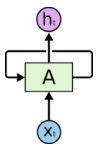
\includegraphics[scale=0.7]{../figs/rnn/loop.png}	
\caption{Input Output loop in RNN}
\label{fig:RNN_Loop} 
\end{figure}

Because of this property, RNNs have been widely used in the fields of sequence modelling \cite{gru_evaluation}, natural language and speech processing \cite{google_speech}. RNNs are also very powerful than some of its other counterparts like ANNs and CNNs because unlike them, the dimensions of the input and output vectors for RNNs can be of arbitrary dimension \cite{gru_evaluation}, depending on the length of the sequence itself.

\begin{figure}[!h]
\centering
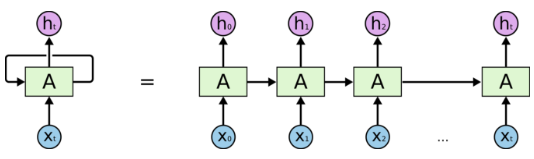
\includegraphics[scale=0.5]{../figs/rnn/unrolled.png}	
\caption{Unrolled Recurrent Neural Network}
\label{fig:RNN_Unrolled} 
\end{figure}

The motivating idea behind RNN is to process a set of input value and store some information derived from it in its own memory called the internal or hidden state. The internal state is updated at every time step using different weight matrices and activation functions depending on the type of architecture used. This internal state is dependent on the current timestep input and internal state from the previous timestep, however the output value of the current timestep is calculated using the current internal state \cite{gru_translation}. This kind of relationship can be formulated mathematically as follows:

\begin{equation}
h_{t} = f(h_{t-1}, x_t)
\end{equation}

Here $h_t$ represents the internal state of the current cell or $t^{th}$ cell, $x_t$ represents the $t^{th}$ input and $h_{t-1}$ represents the ${t-1}^{th}$ cell's internal state. This kind of relationship among the input, internal and output values in a RNN cell is what makes them very apt for modeling the intricate dependencies in a time series.

For this project, we are considering several different types of architecture of RNNs for the problem and all of these architectures usally differ in the computations for the internal state and the output.

\subsubsection{Vanilla RNN}
Vanilla RNNs are the most basic form of RNNs. A Vanilla RNN cell as depicted in Figure \ref{fig:Vanilla_RNN_Arch}, only has one $\tanh$ layer to compute the internal state. This cell only comprises of two sets of computation, one for the internal state and one for the output. The feedforward equations for the Vanilla RNN cell are as follows:

\begin{equation}
h_{t} = \tanh(W_{hh}h_{t-1} + W_{xh}x_t)
\end{equation}
\begin{equation}
y_{t} = W_{hy}h_{t}
\end{equation}

Vanilla RNNs are easy to train because of less number of parameters overall and are easy to apply for problems like classification on top of a sequence of values. 

% Dont need this sentence:
%This generally involves using fully connected layers on top of the outputs of the Vanilla RNN cell and using some kind of activation function in those fully connected layers. 

\begin{figure}[!h]
\centering
\includegraphics[scale=0.20]{../figs/vrnn/diagram.png}	
\caption{Vanilla RNN Cell Architecture}
\label{fig:Vanilla_RNN_Arch} 
\end{figure}

However, one of the biggest disadvantage of using Vanilla RNN is that they are not the best tools for modelling long sequences. Vanilla RNNs are prone to a phenomenen called Vanishing Gradients \cite{vanishing_gradient} \cite{lstm_intro}. Vanishing Gradients refer to the property when the gradient change for the weights in a neural networks are vanishingly small and start approaching the value $0$. Because of this problem the network effectively stops to train/learn. The problem of Vanishing Gradient stems from the fact that different activation functions like $\tanh$ have a gradient value in range: $(0, 1)$. When using the chain rule to calculate the gradient change in earlier layers, the continous multiplication of these small gradient values leads to an exponential decrease in gradient value leading to very small gradient updates.

% Done, added the citation
% Insert the citation for the vanishing gradients as follows: The problem was explored in depth by Hochreiter (1991) [German] and Bengio, et al. (1994), who found some pretty fundamental reasons why it might be difficult.

\subsubsection{Long Short Term Memory (LSTM)}

Long Short Term Memory networks – usually just called “LSTMs” – are a special kind of RNN, capable of learning long-term dependencies. They were introduced by \cite{lstm_intro} to specifically model long term dependencies in a sequence and to combat the problem of vanishing and exploding gradients. Remembering information for long periods of time is practically their default behavior, unlike Vanilla RNN's which struggle to learn long term dependencies.

\begin{figure}[!h]
\centering
\includegraphics[scale=0.40]{../figs/lstm/diagram.png}	
\caption{LSTM Cell Architecture}
\label{fig:LSTM_Arch} 
\end{figure}

Unlike, Vanilla RNNs, LSTM cell \cite{lstm_intro} have four layers of networks interacting in a very special way as can be seen in Figure \ref{fig:LSTM_Arch}. This structure is what makes them combat the problem of vanishing gradient also makes them on the best choices for modelling accoustics \cite{google_accoustics} and for modelling speech \cite{google_speech}.

The key to LSTMs is the \textbf{cell state}, which is different from the hidden/internal state, the horizontal line running through the top of the diagram. This line ensures smooth back propogation of the gradient values by providing a bypass to the gradient values without becoming vanishingly small. Apart from the current cell state, LSTM also includes connections of its input through different gates called the forget, input and output gates. These gates determine what information is persisted, thrown away and added to the current cell state and the internal state. The interaction between the inputs and different gates can be mathematically written as follows:
\begin{equation}
f_{t} = \sigma(W_f\cdot[h_{t-1}, x_t] + b_f)
\end{equation}
\begin{equation}
i_{t} = \sigma(W_i\cdot[h_{t-1}, x_t] + b_i)
\end{equation}
\begin{equation}
\bar{C}_t = \tanh(W_C\cdot[h_{t-1}, x_t] + b_C)
\end{equation}
\begin{equation}
C_t = f_t \cdot C_{t-1} + i_t \cdot \bar{C}_t
\end{equation}
\begin{equation}
o_t = \sigma(W_o[h_{t-1}, x_t] + b_o)
\end{equation}
\begin{equation}
h_t = o_t \cdot \tanh(C_t)
\end{equation}


Here $\sigma$ represents the sigmoid function. %$\sigma(x) = \frac{1}{1 + e^{-x}}$

%\todo{IF TIME PERMITS, WRITE ABOUT PEEPHOLE CONNECTIONS}


% LSTM Theory
%The first step in our LSTM is to decide what information we’re going to throw away from the cell state. This decision is made by a sigmoid layer called the “forget gate layer.” It looks at $h_{t−1}$ and $x_t$, and outputs a number between 0 and 1 for each number in the cell state $C_{t−1}$. A 1 represents “completely keep this” while a 0 represents “completely get rid of this”.
%The next step is to decide what new information we’re going to store in the cell state. This has two parts. First, a sigmoid layer called the “input gate layer” decides which values we’ll update. Next, a tanh layer creates a vector of new candidate values, $\bar{C}_t$, that could be added to the state. In the next step, we’ll combine these two to create an update to the state.
%It’s now time to update the old cell state, $C_{t−1}$, into the new cell state $C_t$. The previous steps already decided what to do, we just need to actually do it. We multiply the old state by $f_t$, forgetting the things we decided to forget earlier. Then we add $i_t \cdot \bar{C}_t$. This is the new candidate values, scaled by how much we decided to update each state value.
%Finally, we need to decide what we’re going to output. This output will be based on our cell state, but will be a filtered version. First, we run a sigmoid layer which decides what parts of the cell state we’re going to output. Then, we put the cell state through $\tanh$ (to push the values to be between −1 and 1) and multiply it by the output of the sigmoid gate, so that we only output the parts we decided to.


\subsubsection{Gated Recurrent Unit}

LSTMs are extremely popular in modelling long term dependencies in audio, text, speech data. However because of its intricate structure it is harder to train. The number of parameters in LSTM is much more than Vanilla RNN, which makes it more time consuming to train and often harder to reach a state of convergence. A slightly more dramatic variation on the LSTM is the Gated Recurrent Unit, or GRU, introduced by Cho, et al. (2014) \cite{gru_translation}. 

\begin{figure}[!h]
\centering
\includegraphics[scale=0.50]{../figs/gru/diagram.png}	
\caption{GRU Cell Architecture}
\label{fig:GRU_Arch} 
\end{figure}

GRU essentially uses LSTM arhcitecture to combat the problem of vanishing gradients, but it combines the forget and input gates into a single “update gate” and also merges the cell state and hidden state, effectively reducing the number of learnable parameters. Because of this change in architecture LSTM and GRU differ in the way they calculate the output values and also in the internal state that they remember \cite{gru_evaluation}. The changes in the architecture are visible in Figure: \ref{fig:GRU_Arch}. The resulting model is simpler than standard LSTM models, and has been growing increasingly popular, especially in the fields of machine translation \cite{gru_translation} and sequence modelling \cite{gru_evaluation}. The new feedforward equations for GRU are as follows:
\begin{equation}
z_t = \sigma(W_z \cdot [h_{t-1}, x_t])
\end{equation}
\begin{equation}
r_t = \sigma(W_r \cdot [h_{t-1}, x_t])
\end{equation}
\begin{equation}
\bar{h}_t = \tanh(W \cdot [r_t \cdot h_{t-1}, x_t])
\end{equation}
\begin{equation}
h_t = (1 - z_t) \cdot h_{t-1} + z_t \cdot \bar{h}_{t}
\end{equation}
Here $\sigma$ represents the sigmoid function.

\subsubsection{Bidirectional LSTM}

All the architectures we have looked uptil now involves just looking at information from the previous context or from past. However sometimes it is better to use the information from past and future context at once. If we already have the whole series it is better to use the historical and future context for better modelling of the data. Bidirectional LSTM implement this kind of behavior by connecting two hidden layers of opposite directions to the same output \cite{blstm_intro}. The architecture of BLSTMs as can be seen in Figure: \ref{fig:BLSTM_Arch} hence looks a little different because they have two connections for each LSTM cell from both sides. These connections update the internal state by accumulating information from historical and future context and then the internal states are used to to calculate the final output. Because of this kind of architecture BLSTM are perfect for places where more context is necessary to remove ambiguity, like in English language \cite{blstm_intro}. BLSTM are especially useful when the context of the input is needed, for example, in handwriting recognition, speech recognition \cite{bidirectional_lstm_speech}, speech synthesis, phenome classification and protein synthesis \cite{blstm_protein}. 

\begin{figure}[!h]
\centering
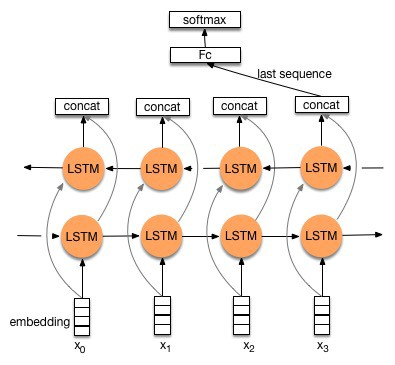
\includegraphics[scale=0.50]{../figs/blstm/diagram.jpeg}	
\caption{BLSTM Architecture}
\label{fig:BLSTM_Arch} 
\end{figure}


\subsection{Convolutional Neural Networks (CNN)}

% Give a little introduction about how CNNs work and why are they use. Show how they were designed to extract local features and how they learn it. This section will cover the basics of convolution, activations like RELU and things like max pooling
CNNs are another type of artificial neural networks designed specifically for the purpose of processing visual data like images. In today's time, CNN based architectures have been widely used in fields like Image Classification \cite{ilsvrc} and Object Detection. The motivating idea behind CNNs is that visual data has an inherent local structure such that values which are closer to each other tend to influence each other \cite{imagenet_original}. To understand this, we can take the example of an image of a scenery. We know pixels representing the grass in the image tend to be similar to each other (mostly green). To exploit this property, CNNs use something called Convolutions, which refer to a weighted sum of values slided over the input to get an output. Convolutions are often referred as Kernels because they are functions/maps/filters which are slided over the input features to get the output features. Because of convolutions CNN's become very powerful because they are automatically able to learn different latent visual features also termed as \textit{"feature maps"}. This property is very useful and powerful and because of this CNNs are able to perform very well on visual data. This property makes CNN's very different from other traditional Machine Learning Algorithms, where the features have to be already specified. Considering the CNN's learn these high dimensional feature maps from the given input we aim to use CNNs to extract these features and then build a neural network model on top of these features to classify the audio dataset. A simple CNN architecture often involves multiple layers of several of these convolution layers. Each of these layers are then seperated by a nonlinearity. One of the most commonly used non linearity is \textbf{Rectified Linear Unit (ReLU)} \cite{imagenet_original}. The biggest advantage of ReLU is that the gradient value for ReLU is either $1$ or $0$, hence either the gradient passes just through the convolution or does not, effectively eliminating the problem of vanishing and exploding gradients.

\begin{figure}[!h]
\centering
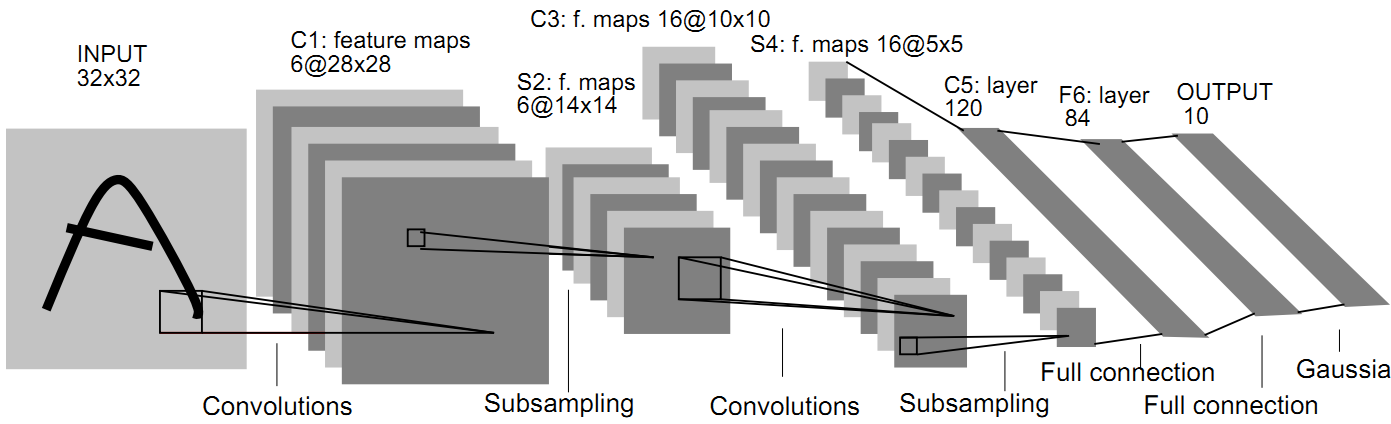
\includegraphics[width=8cm,height=3cm]{../figs/cnn/le_net.png}	
\caption{Le Net \cite{le_net}: One of the earliest successful CNN}
\label{fig:Le_Net_Arch} 
\end{figure}

One of the earliest developed and successful CNNs was developed by Yan Le Cunn \cite{le_net} and trained on the MNIST dataset \ref{fig:Le_Net_Arch}. It was designed to recognise different mathematical digits. This was one of the greatest development in the field of image recognition. After that with the introduction of Imagenet challenge and powerful Graphical Processing units, deeper architectures were developed which exceeded human performance. One of the best models was called Resnet-152, containing 152 hidden layers. The architecture for Resnet-152 was distinct from other architectures because of the added residual connections (Figure: \ref{fig:Resnet_Residual_Arch}, which were again added for smoother flow of the gradient through the network.

\begin{figure}[!h]
\centering
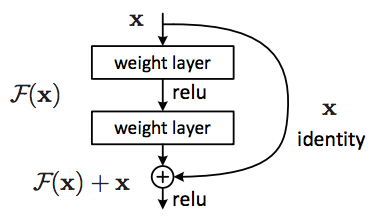
\includegraphics[scale=0.30]{../figs/cnn/resnet_residual.png}	
\caption{Residual Connections in Resnet}
\label{fig:Resnet_Residual_Arch} 
\end{figure}


Because of a lot of stacked convolution layers all the feature maps start learning higher dimensional features which cannot be described beforehand by a human. This is what made it perform exceedingly well. Deeper CNNs are although very powerful but they also become very hard to interpret because as a human it becomes harder to understand what those higher dimensional features represent.

In this project we try to use CNN's for the purpose of exploring how well do they do in processing time dependent data and to understand how well CNNs can learn local features from different images which have been produced by processing an audio signal.

\subsubsection{Stacking}

\begin{figure}[!h]
\centering
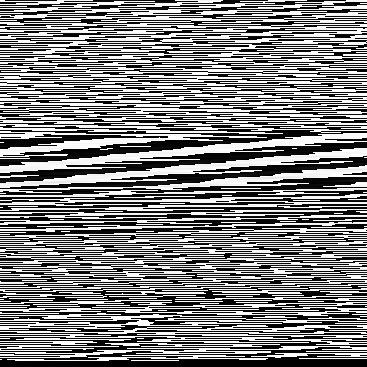
\includegraphics[scale=0.30]{../figs/stacking/sax.jpg}	
\caption{Stacked Image of Saxophone Audio Signal}
\label{fig:Sax_Stack} 
\end{figure}

Because CNN's are specifically designed to handle at least Two Dimensional data, for the terms of this project there are two ways of converting audio signal data (one dimensional) to an image (two dimensional). The first way is termed as stacking because it just refers to splitting an audio signal data vector into equal sized smaller vectors and stacking them on top of one other, hence the name stacking. For the purpose of this project and because CNN's are well suited to process square images, we first \textit{zero-pad} the audio signal data until the length of the vector becomes a perfect square. After this preprocessing, we just reshape the vector to a matrix with first N elements in the first row, then the second N elements in the second row and so on to get a $N$ x $N$ greyscale image. One example of the images I constructed for this project can be seen in Figure: \ref{fig:Sax_Stack}

\subsubsection{Multiresolution Recurrent Plot (MRP)}

Other than stacking there also exist other techniques to convert audio data signals into an image. One of the techinques we are also considering for this project is called Multiresolution Recurrence Plot (MRP). As mentioned in Park et al. \cite{cnn_music_mrp} using MRPs, time series data can be analyzed in the two dimensional space without losing any information. A traditional recurrent plot is used to measure the distance between two different phase trajectories at all different possible timestep combinations. It helps to visualize how a sequence or trajectory occurs again or repeats, which defines the recurrent pattern. The equation behind RPs is as follows:

\begin{equation}
R[i, j] = |{x[i] - x[j]}|
\end{equation}

RPs are very popular for converting time series data into image based data in the field of mediciene. We can use a similar techinque for the case of the instruments and their recordings. However, because different instruments have very different frequency, it becomes important to use different sized window techinques for each recurrent plot from the same instrument so that all instruments and their respective frequency range can be visualized in the plot. MRPs implement this by actually extracting different size of samples from the same time series data and then constructing a RP on top of them. However because CNNs are fixed in terms of the input size, we use pooling layers to get the same size even for different sized input time series sample. Example of a MRP for Saxophone is below.	

\begin{figure}[!h]
\centering
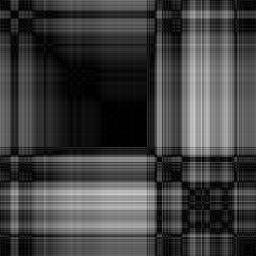
\includegraphics[scale=0.40]{../figs/mrp/sax.jpg}	
\caption{Recurrence Plot for Saxophone}
\label{fig:MRP_Sax} 
\end{figure}


\subsubsection{R-CNN on MRP Images}

Until now, we have talked about how RNNs are a very powerful tool for modelling sequential data because of their innate capabilities of holding memory from past and sometimes even the future data. While on the other hand CNNs are powerful tool for modelling visual data because of their property of learning latent high dimensional features. Considering that our problem works on the concept of Audio Classification/Image recognition such that we already have all the audio data as .wav files and also using the techinque mentioned before about MRP we can also convert our time series data into an image, we are also trying to implement the kind of network used in Aggarwal et al. \cite{cnn_rnn_sleep_staging}
which combines CNNs and RNNs. The network mentioned in \cite{cnn_rnn_sleep_staging} works well for Sleep staging, however we will change the architecture a little bit to suit our problem. We will apply CNN on the MRP images to learn various latent high dimensional features and pass the information about these features to an LSTM cell as its initial internal state. We will be using LSTM and not GRU, because it can be seen that LSTM cells have been already used in Audio Classification \cite{lstm_music_genre} and performed very well.


\begin{thebibliography}{99}

\bibitem{IRMAS_Dataset} Bosch, Juan J., et al. "A Comparison of Sound Segregation Techniques for Predominant Instrument Recognition in Musical Audio Signals." ISMIR. 2012.

\bibitem{google_accoustics} Sak, Haşim, Andrew Senior, and Françoise Beaufays. "Long short-term memory recurrent neural network architectures for large scale acoustic modeling." Fifteenth annual conference of the international speech communication association. 2014.

\bibitem{google_speech} Sak, Haşim, Andrew Senior, and Françoise Beaufays. "Long short-term memory based recurrent neural network architectures for large vocabulary speech recognition." arXiv preprint arXiv:1402.1128 (2014).

\bibitem{imagenet_original} Krizhevsky, Alex, Ilya Sutskever, and Geoffrey E. Hinton. "Imagenet classification with deep convolutional neural networks." Advances in neural information processing systems. 2012.

\bibitem{bidirectional_lstm_speech} Graves, Alex, and Navdeep Jaitly. "Towards end-to-end speech recognition with recurrent neural networks." International Conference on Machine Learning. 2014.

\bibitem{renet} Visin, Francesco, et al. "Renet: A recurrent neural network based alternative to convolutional networks." arXiv preprint arXiv:1505.00393 (2015).

\bibitem{gru_evaluation} Chung, Junyoung, et al. "Empirical evaluation of gated recurrent neural networks on sequence modeling." arXiv preprint arXiv:1412.3555 (2014).

\bibitem{gru_translation} Cho, Kyunghyun, et al. "On the properties of neural machine translation: Encoder-decoder approaches." arXiv preprint arXiv:1409.1259 (2014).

\bibitem{lstm_sequence_modelling} Graves, Alex. "Generating sequences with recurrent neural networks." arXiv preprint arXiv:1308.0850 (2013).

\bibitem{cnn_rnn_sleep_staging} Aggarwal, Karan, et al. "A Structured Learning Approach with Neural Conditional Random Fields for Sleep Staging."

\bibitem{cnn_music_mrp} Park, Taejin, and Taejin Lee. "Musical instrument sound classification with deep convolutional neural network using feature fusion approach." arXiv preprint arXiv:1512.07370 (2015).

\bibitem{lstm_music_genre} Tang, Chun Pui, et al. "Music Genre classification using a hierarchical Long Short Term Memory (LSTM) model." (2018).

\bibitem{vanishing_gradient} Pascanu, Razvan, Tomas Mikolov, and Yoshua Bengio. "On The Difficulty Of Training Recurrent Neural Networks." Arxiv.org. N. p., 2012. Web. 13 Dec. 2018.

\bibitem{lstm_intro} Hochreiter, Sepp, and Jürgen Schmidhuber. "Long short-term memory." Neural computation 9.8 (1997): 1735-1780.

\bibitem{blstm_intro} Yu, Zhou, et al. "Using bidirectional LSTM recurrent neural networks to learn high-level abstractions of sequential features for automated scoring of non-native spontaneous speech." Automatic Speech Recognition and Understanding (ASRU), 2015 IEEE Workshop on. IEEE, 2015.

\bibitem{blstm_protein} Thireou, Trias, and Martin Reczko. "Bidirectional long short-term memory networks for predicting the subcellular localization of eukaryotic proteins." IEEE/ACM Transactions on Computational Biology and Bioinformatics (TCBB) 4.3 (2007): 441-446.

\bibitem{ilsvrc} Olga Russakovsky*, Jia Deng*, Hao Su, Jonathan Krause, Sanjeev Satheesh, Sean Ma, Zhiheng Huang, Andrej Karpathy, Aditya Khosla, Michael Bernstein, Alexander C. Berg and Li Fei-Fei. (* = equal contribution) ImageNet Large Scale Visual Recognition 

\bibitem{le_net} Y. LeCun, L. Bottou, Y. Bengio, and P. Haffner. Gradient-based learning applied to document recognition. Proceedings of the IEEE, november 1998

\end{thebibliography}

\end{document}
